
%(BEGIN_QUESTION)
% Copyright 2006, Tony R. Kuphaldt, released under the Creative Commons Attribution License (v 1.0)
% This means you may do almost anything with this work of mine, so long as you give me proper credit

Anta at du skulle koble en HART-kompatibel transmitter til en indikator som ikke tålte de høyfrekvente HART-kommunikasjonssignalene. Vis hvor du ville plassert en HART-{\it filter}krets i denne 4-20 mA-sløyfen for å hindre at de høyfrekvente signalene når indikatoren, og hva denne filterkretsen skulle bestå av:

$$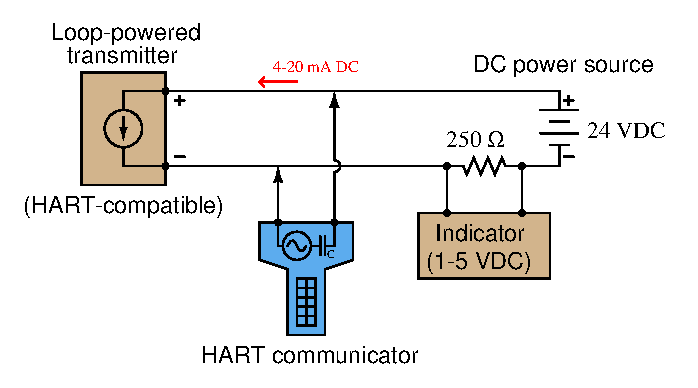
\includegraphics[width=15.5cm]{i01398x01.eps}$$

\underbar{file i01398}
%(END_QUESTION)





%(BEGIN_ANSWER)

Uansett hvordan du planlegger å filtrere HART-signalene, motstå fristelsen til å gjøre dette:

$$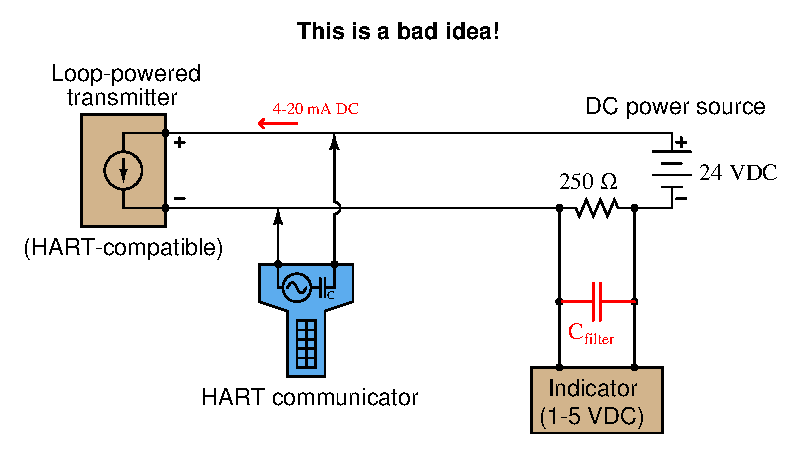
\includegraphics[width=15.5cm]{i01398x04.eps}$$

Selv om en kondensator over indikatorens terminaler vil lede høyfrekvente AC HART-signaler utenom indikatoren, vil den også kortslutte HART-dataene fullstendig slik at transmitteren og kommunikatoren ikke kan snakke sammen!

Jeg lar deg finne en bedre metode for HART-signalfiltrering -- en som hindrer HART-frekvensene i å nå indikatoren uten å slå ut HART-signalene i resten av nettverket.

%(END_ANSWER)





%(BEGIN_NOTES)

Det finnes to grunnleggende alternativer: {\it blokkere} eller {\it lede utenom}. Først ``blokkere''-alternativet:

$$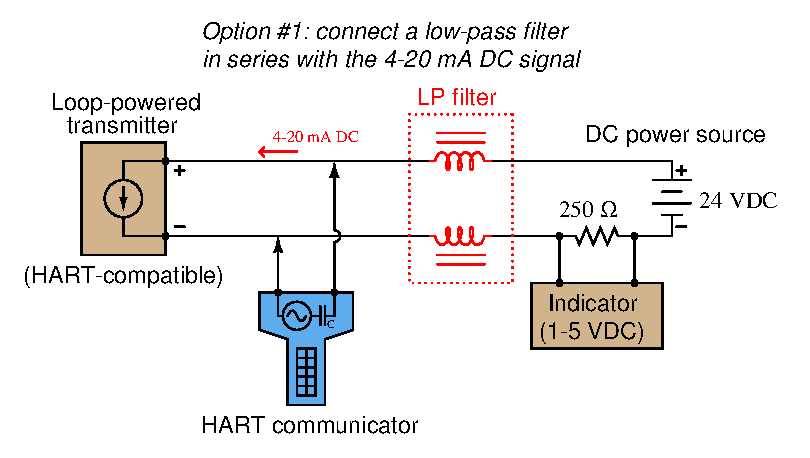
\includegraphics[width=15.5cm]{i01398x03.eps}$$

\vskip 10pt

\filbreak

Deretter ``lede utenom''-alternativet:

$$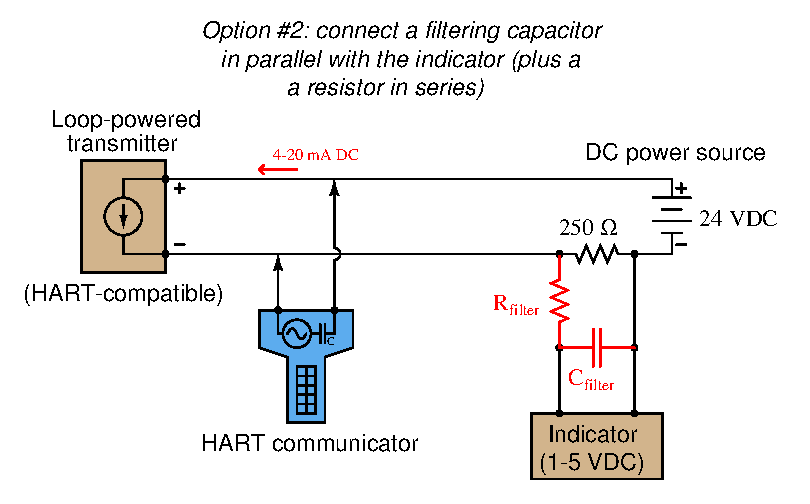
\includegraphics[width=15.5cm]{i01398x02.eps}$$

%INDEX% Fieldbus, HART: filter circuit

%(END_NOTES)

